\section{Geometric distributed values}
For the geometric distribution the chosen default value is $p=0.001$.
This results in an expected value of 1000 which is the same as for the binomial distribution in the last subsection.
This should make the results more comparable.
The maximum value is theoretically not limited but for the implementation in Java the maximum value was set to the maximum value of a long value $= 2^{63}-1 = 9,223,372,036,854,775,807$.
Without this maximum the value might overflow and instead be negative with high absolute value.
Figure~\ref{fig:geoDistExample} shows a random geometric distributed input.
The span of all values is way higher than for the binomial distribution, although they have same expected value.
Here the values are not in the interval $[800,1200]$ but rather between 0 and 9000.
The theoretical limitation of the values being at most $2^{63}-1$ seems to not have an influence on the results.
The geometric distribution does not only have low values close or equal to 1 but also has mostly values that are very small.
This should lead to 1-bit flips being effective as the small values can remove the small differences.
Because there are so many small values moving only one bit might be better than switching two elements.
\begin{figure}[h]
      \caption{Distribution of a random geometric input}
      \centering
      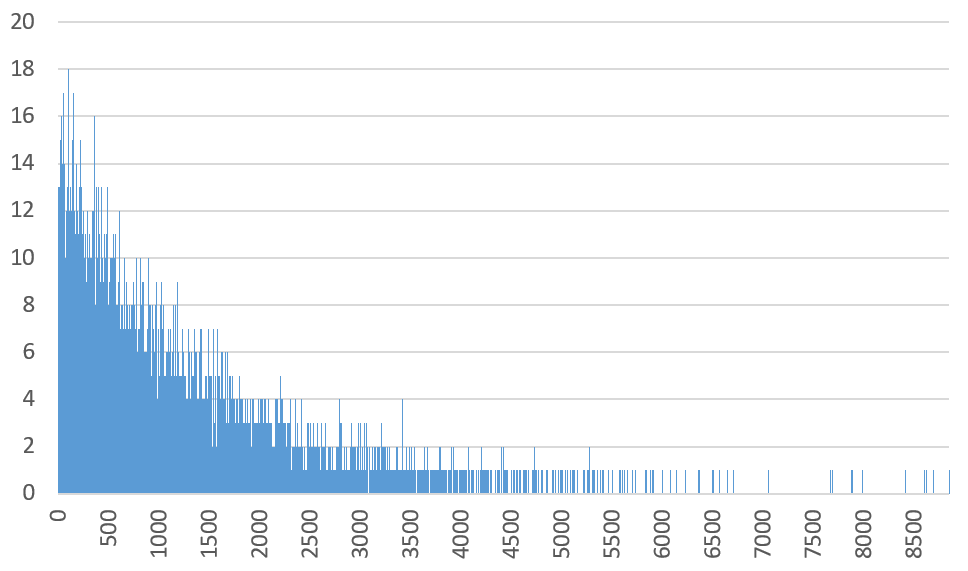
\includegraphics[width=0.7\textwidth]{figures/images/numberGenerator/geometricDistributionForp0_001.png}\label{fig:geoDistExample}
\end{figure}
\subsection{RLS Comparison}
\makebox[\linewidth]{
\begin{tabular}{lp{3cm}p{6cm}p{6cm}}
\begin{tabular}[h]{cccccccc}
algo type&            \RLSN&     \RLSR&     \RLSR&     \RLSN&     \RLSR&     \RLSN&       RLS\\
algo param&             b=2&       s=3&       s=4&       b=3&       s=2&       b=4&         -\\
avg mut/change&       2.000&     1.996&     2.476&     3.000&     1.502&     4.000&     1.000\\
avg mut/step&         2.000&     2.000&     2.500&     3.000&     1.500&     4.000&     1.000\\
\hline
total avg count&     83,118&   104,748&   105,513&   112,223&   114,486&   121,927& 2,443,567\\
avg eval count&      83,118&   104,748&   105,513&   112,223&   114,486&   121,927&    45,834\\
max eval count&     778,110& 1,453,252&   898,974& 1,377,471&   915,268&   816,633&   485,275\\
min eval count&         197&       126&        45&       212&       271&       155&       128\\
\hline
fail ratio&           0.000&     0.000&     0.000&     0.000&     0.000&     0.000&     0.447\\
avg fail dif&             -&         -&         -&         -&         -&         -&         1\\
\end{tabular}
\end{tabular}
}


For these inputs the variants of the RLS perform differently to the binomial input.
The only similarity is the RLS being the only algorithm that did not find an optimal solution for every input.
If the RLS did find an optimal solution in those 21 cases it instead might be the best RLS variant.
The other algorithms are ranked by their probability of flipping only one bit.
This means at first the three \RLSR[s] variants from 2 to 3 to 4 and then the same for the \RLSN[b] variants.
So it does seem like moving mostly one element at once is better for the geometric input in comparison to two elements for the binomial distribution.
In the 21 cases where the RLS did not find an optimal solution it was most likely stuck in a local optimum where no small value was left.

\subsection{(1+1) EA Comparison}
\makebox[\linewidth]{
\begin{tabular}{lp{3cm}p{6cm}p{6cm}}
\begin{tabular}[h]{ccccccccc}
algo type&          (1+1) EA&   (1+1) EA&   (1+1) EA&   (1+1) EA&      (1+1) EA&   (1+1) EA&   (1+1) EA&   (1+1) EA\\
algo param&           3/n&     4/n&     2/n&     5/n&       -&    10/n&    50/n&   100/n\\
avg mut/change&     3.101&   3.968&   2.343&   4.859&   1.698&   9.732&  49.544&  99.494\\
avg mut/step&       2.999&   4.003&   2.002&   4.999&   1.001&   9.998&  49.998&  99.997\\
\hline
total avg count&      646&     701&     706&     857&   1,123&   1,508&   8,175&  15,485\\
avg eval count&       646&     701&     706&     857&   1,123&   1,508&   8,175&  15,485\\
max eval count&     5,346&   5,692&   3,415&   5,572&   7,001&  12,112&  52,831& 145,269\\
min eval count&        23&       4&      30&       9&      23&      14&      27&      69\\
\hline
fails&                  0&       0&       0&       0&       0&       0&       0&       0\\
fail ratio&         0.000&   0.000&   0.000&   0.000&   0.000&   0.000&   0.000&   0.000\\
avg fail dif&           -&       -&       -&       -&       -&       -&       -&       -\\
\end{tabular}
\end{tabular}
}


The results for the (1+1) EA are similar to the results of the RLS. From mutation rate $2/n$ on the runtime increases with rising mutation rate.
The only part that does not fit into the theory of 1 bit flips being superior is the mutation rate $2/n$ performing better than the standard $1/n$.
All variants reach an optimal solution within the given limit for the number of iterations.
\subsection{pmut Comparison}
\makebox[\linewidth]{
\scriptsize
\begin{tabular}{lp{3cm}p{6cm}p{6cm}}
\begin{tabular}[h]{m{2.5cm}m{0,40cm}m{0,40cm}m{0,40cm}m{0,40cm}m{0,40cm}m{0,40cm}m{0,40cm}m{0,40cm}m{0,40cm}m{0,40cm}m{0,40cm}m{0,40cm}m{0,40cm}m{0,40cm}m{0,40cm}m{0,40cm}m{0,40cm}m{0,40cm}}
\multicolumn{1}{c}{algo type}&\multicolumn{2}{c}{            pmut}&\multicolumn{2}{c}{     pmut}&\multicolumn{2}{c}{     pmut}&\multicolumn{2}{c}{     pmut}&\multicolumn{2}{c}{     pmut}&\multicolumn{2}{c}{     pmut}&\multicolumn{2}{c}{     pmut}&\multicolumn{2}{c}{     pmut}&\multicolumn{2}{c}{     pmut}\\
\multicolumn{1}{c}{algo param}&\multicolumn{2}{c}{           3.25}&\multicolumn{2}{c}{     3.00}&\multicolumn{2}{c}{     2.75}&\multicolumn{2}{c}{     2.50}&\multicolumn{2}{c}{     2.25}&\multicolumn{2}{c}{     2.00}&\multicolumn{2}{c}{     1.75}&\multicolumn{2}{c}{     1.50}&\multicolumn{2}{c}{     1.25}\\
\multicolumn{1}{c}{avg mut/change}&\multicolumn{2}{c}{      1.583}&\multicolumn{2}{c}{    1.737}&\multicolumn{2}{c}{    2.002}&\multicolumn{2}{c}{    2.423}&\multicolumn{2}{c}{    3.303}&\multicolumn{2}{c}{    5.830}&\multicolumn{2}{c}{   12.519}&\multicolumn{2}{c}{   30.910}&\multicolumn{2}{c}{   73.182}\\
\multicolumn{1}{c}{avg mut/step}&\multicolumn{2}{c}{        1.729}&\multicolumn{2}{c}{    1.934}&\multicolumn{2}{c}{    2.274}&\multicolumn{2}{c}{    2.895}&\multicolumn{2}{c}{    4.360}&\multicolumn{2}{c}{    8.452}&\multicolumn{2}{c}{   22.278}&\multicolumn{2}{c}{   70.532}&\multicolumn{2}{c}{  224.421}\\
\hline
\multicolumn{1}{c}{avg eval count}&\multicolumn{2}{c}{        540}&\multicolumn{2}{c}{      569}&\multicolumn{2}{c}{      594}&\multicolumn{2}{c}{      641}&\multicolumn{2}{c}{      712}&\multicolumn{2}{c}{      808}&\multicolumn{2}{c}{      967}&\multicolumn{2}{c}{    1,285}&\multicolumn{2}{c}{    2,081}\\
\multicolumn{1}{c}{max eval count}&\multicolumn{2}{c}{      3,110}&\multicolumn{2}{c}{    2,891}&\multicolumn{2}{c}{    3,504}&\multicolumn{2}{c}{    3,896}&\multicolumn{2}{c}{    5,152}&\multicolumn{2}{c}{    4,274}&\multicolumn{2}{c}{    5,610}&\multicolumn{2}{c}{    6,190}&\multicolumn{2}{c}{   14,984}\\
\multicolumn{1}{c}{min eval count}&\multicolumn{2}{c}{         22}&\multicolumn{2}{c}{        9}&\multicolumn{2}{c}{       36}&\multicolumn{2}{c}{       25}&\multicolumn{2}{c}{       28}&\multicolumn{2}{c}{       27}&\multicolumn{2}{c}{       27}&\multicolumn{2}{c}{       13}&\multicolumn{2}{c}{       33}\\
\hline
\multicolumn{1}{c}{fail ratio}&\multicolumn{2}{c}{          0.000}&\multicolumn{2}{c}{    0.000}&\multicolumn{2}{c}{    0.000}&\multicolumn{2}{c}{    0.000}&\multicolumn{2}{c}{    0.000}&\multicolumn{2}{c}{    0.000}&\multicolumn{2}{c}{    0.000}&\multicolumn{2}{c}{    0.000}&\multicolumn{2}{c}{    0.000}\\
\hline
\multicolumn{1}{c}{p-value}&&\multicolumn{2}{c}{0.0000}&\multicolumn{2}{c}{0.0000}&\multicolumn{2}{c}{0.0000}&\multicolumn{2}{c}{0.0000}&\multicolumn{2}{c}{0.0000}&\multicolumn{2}{c}{0.0000}&\multicolumn{2}{c}{0.0000}&\multicolumn{2}{c}{0.0000}\\
&&&&&&&&&&&&&&&&&&\end{tabular}
\end{tabular}
}


The results for the $pmut_\beta$ operator are even more clear than for the (1+1) EA.\
With decreasing values for $\beta$ the amount of flipped bits per step increases.
The performance decreases as well with decreasing values for $\beta$ which fits into the theory of one bit flips being better for geometric distributed inputs.
The number of repetitions of the algorithm might simply be too small to make the small difference in the performance between the two values visible.
The difference in the performance for the $pmut_\beta$ operator is not as drastic as for the (1+1) EA.
Only $\beta=1.5$ and $\beta=1.25$ perform significantly worse the next best value.

\subsection{Comparison of the best variants}
% \makebox[\linewidth]{
\begin{tabular}{lp{3cm}p{6cm}p{6cm}}
\begin{tabular}[h]{cccc}
algo type&            RLS&    pmut&      EA\\
algo param&             -&    3.25&       -\\
avg mut/change&     1.000&   1.287&   1.272\\
avg mut/step&       1.000&   1.729&   1.000\\
\hline
avg eval count&    91,171& 143,121& 231,082\\
max eval count&   153,143& 227,737& 446,942\\
min eval count&    65,783&  93,602& 165,818\\
\hline
fail ratio&         0.000&   0.000&   0.000\\
\end{tabular}
\end{tabular}
}

% 
The setup for the evaluation of lower values for $n$ is mostly the same except for having a fixed time limit of 100,000 instead of using 50,000 as the limit.
The first try was executed with 50,000 but there the algorithms performed too bad for $n=20$.
Therefore in the second attempt the step limit was increased to 100,000.
The first table lists the number of runs where the different algorithms did not find the optimal solution within the time limit.

\begin{tabular}[h]{ccccccccc}
fails in 1000 runs&20&50&100&500&1000&5000&10000&50000\\\hline
RLS&984&773&411&1&0&0&0&0\\
\RLSR[2]&890&241&14&0&0&0&0&0\\
(1+1) EA (1$/n$)&711&75&5&0&0&0&0&0\\
(1+1) EA (2$/n$)&541&14&0&0&0&0&0&0\\
pmut (3.0)&566&63&4&0&0&0&0&0\\
pmut (3.25)&587&63&7&0&0&0&0&0\\
\end{tabular}


For small inputs the geometric distributed input seems to have inputs without a perfect partition because there were many iterations where neither of the algorithms found an optimal solution within the time limit.
It is still likely to have a perfect partition even for the small values in comparison to other distributions which follow afterwards.
Many algorithms especially the variants of the RLS seem to be likely to get stuck in a local optimum.
The (1+1) EA finds an optimum in most of the runs, so the geometric distributed inputs also seem to be likely to have a perfect partition for small values.
They definitely are harder to solve for smaller input sizes than the binomial inputs, but they still have a perfect partition most times.
The next table visualises the average number of iterations the algorithms needed for finding an optimal solution if the algorithm managed to do so.

\begin{tabular}[h]{ccccccccc}
avg&20&50&100&500&1000&5000&10000&50000\\\hline
RLS&32&79&153&579&950&1859&1922&1797\\
\RLSR[2]&391&2124&5005&4218&3530&2362&2160&2229\\
(1+1) EA (1$/n$)&22471&18343&12834&8342&6511&3815&3458&3371\\
(1+1) EA (2$/n$)&16360&9243&6452&4503&4020&3171&3141&3133\\
pmut (3.25)&23440&15929&9658&5644&4406&2434&2162&2172\\
pmut (3.0)&21901&14696&9186&5222&4150&2510&2208&2213\\
\end{tabular}


The variants of the (1+1) EA and of the $pmut$ algorithm seem to take about 20,000 iterations for $n=20$ if they manage to find the optimal solution.
They also perform better and better the bigger the input gets.
This is probability caused by the many additional small values that can be used for smaller adjustments to the fitness.
Also a really high value does not have as much of an effect, because there are possibly other larger values which cancel each other out, if they are in different bins.
The standard (1+1) EA does not only find a perfect partition less often, it also needs more iterations on average if it does.
So the (1+1) EA with $p_m=2/n$ performs indeed better for every input size.
The last table again lists the total average number of steps.

\begin{tabular}[h]{ccccccccc}
total avg&20&50&100&500&1000&5000&10000&50000\\\hline
RLS&99470&93459&74385&3474&447&389&421&555\\
\RLSR[2]&96305&63088&19364&815&589&565&595&699\\
(1+1) EA (1$/n$)&89444&52886&21141&1410&869&850&875&1046\\
(1+1) EA (2$/n$)&79603&37214&14107&1302&992&942&957&1055\\
pmut (3.25)&84226&48403&18280&930&542&526&546&642\\
pmut (3.0)&82474&46286&17825&917&576&548&573&668\\
\end{tabular}


The RLS is only an option if the input is large enough ($n \ge 10,000$). For smaller input sizes especially for $n \le 100$ choosing the (1+1) EA with mutation rate $2/n$ seems like the best choice. For larger values this (1+1) EA does not find an optimal solution the fastest but is still fast enough to be a viable option. Another rather save option is $pmut_{3.25}$. This algorithm performs worse for $n \le 100$ but is still good in comparison to the other algorithms. For $n \ge 1000$ $pmut_{3.25}$ starts to outperform the best version of the (1+1) EA and almost all other researched algorithms.
